% Options for packages loaded elsewhere
\PassOptionsToPackage{unicode}{hyperref}
\PassOptionsToPackage{hyphens}{url}
%
\documentclass[
  12pt,
]{article}
\usepackage{amsmath,amssymb}
\usepackage{iftex}
\ifPDFTeX
  \usepackage[T1]{fontenc}
  \usepackage[utf8]{inputenc}
  \usepackage{textcomp} % provide euro and other symbols
\else % if luatex or xetex
  \usepackage{unicode-math} % this also loads fontspec
  \defaultfontfeatures{Scale=MatchLowercase}
  \defaultfontfeatures[\rmfamily]{Ligatures=TeX,Scale=1}
\fi
\usepackage{lmodern}
\ifPDFTeX\else
  % xetex/luatex font selection
\fi
% Use upquote if available, for straight quotes in verbatim environments
\IfFileExists{upquote.sty}{\usepackage{upquote}}{}
\IfFileExists{microtype.sty}{% use microtype if available
  \usepackage[]{microtype}
  \UseMicrotypeSet[protrusion]{basicmath} % disable protrusion for tt fonts
}{}
\makeatletter
\@ifundefined{KOMAClassName}{% if non-KOMA class
  \IfFileExists{parskip.sty}{%
    \usepackage{parskip}
  }{% else
    \setlength{\parindent}{0pt}
    \setlength{\parskip}{6pt plus 2pt minus 1pt}}
}{% if KOMA class
  \KOMAoptions{parskip=half}}
\makeatother
\usepackage{xcolor}
\usepackage[margin=1in]{geometry}
\usepackage{longtable,booktabs,array}
\usepackage{calc} % for calculating minipage widths
% Correct order of tables after \paragraph or \subparagraph
\usepackage{etoolbox}
\makeatletter
\patchcmd\longtable{\par}{\if@noskipsec\mbox{}\fi\par}{}{}
\makeatother
% Allow footnotes in longtable head/foot
\IfFileExists{footnotehyper.sty}{\usepackage{footnotehyper}}{\usepackage{footnote}}
\makesavenoteenv{longtable}
\usepackage{graphicx}
\makeatletter
\def\maxwidth{\ifdim\Gin@nat@width>\linewidth\linewidth\else\Gin@nat@width\fi}
\def\maxheight{\ifdim\Gin@nat@height>\textheight\textheight\else\Gin@nat@height\fi}
\makeatother
% Scale images if necessary, so that they will not overflow the page
% margins by default, and it is still possible to overwrite the defaults
% using explicit options in \includegraphics[width, height, ...]{}
\setkeys{Gin}{width=\maxwidth,height=\maxheight,keepaspectratio}
% Set default figure placement to htbp
\makeatletter
\def\fps@figure{htbp}
\makeatother
\setlength{\emergencystretch}{3em} % prevent overfull lines
\providecommand{\tightlist}{%
  \setlength{\itemsep}{0pt}\setlength{\parskip}{0pt}}
\setcounter{secnumdepth}{5}
\newlength{\cslhangindent}
\setlength{\cslhangindent}{1.5em}
\newlength{\csllabelwidth}
\setlength{\csllabelwidth}{3em}
\newlength{\cslentryspacingunit} % times entry-spacing
\setlength{\cslentryspacingunit}{\parskip}
\newenvironment{CSLReferences}[2] % #1 hanging-ident, #2 entry spacing
 {% don't indent paragraphs
  \setlength{\parindent}{0pt}
  % turn on hanging indent if param 1 is 1
  \ifodd #1
  \let\oldpar\par
  \def\par{\hangindent=\cslhangindent\oldpar}
  \fi
  % set entry spacing
  \setlength{\parskip}{#2\cslentryspacingunit}
 }%
 {}
\usepackage{calc}
\newcommand{\CSLBlock}[1]{#1\hfill\break}
\newcommand{\CSLLeftMargin}[1]{\parbox[t]{\csllabelwidth}{#1}}
\newcommand{\CSLRightInline}[1]{\parbox[t]{\linewidth - \csllabelwidth}{#1}\break}
\newcommand{\CSLIndent}[1]{\hspace{\cslhangindent}#1}
\setlength{\parindent}{4em}
\usepackage{setspace}\doublespacing
\usepackage{placeins}
\usepackage{bbm}
\usepackage{booktabs}
\usepackage{booktabs}
\usepackage{longtable}
\usepackage{array}
\usepackage{multirow}
\usepackage{wrapfig}
\usepackage{float}
\usepackage{colortbl}
\usepackage{pdflscape}
\usepackage{tabu}
\usepackage{threeparttable}
\usepackage{threeparttablex}
\usepackage[normalem]{ulem}
\usepackage{makecell}
\usepackage{xcolor}
\usepackage{siunitx}

  \newcolumntype{d}{S[
    input-open-uncertainty=,
    input-close-uncertainty=,
    parse-numbers = false,
    table-align-text-pre=false,
    table-align-text-post=false
  ]}
  
\ifLuaTeX
  \usepackage{selnolig}  % disable illegal ligatures
\fi
\IfFileExists{bookmark.sty}{\usepackage{bookmark}}{\usepackage{hyperref}}
\IfFileExists{xurl.sty}{\usepackage{xurl}}{} % add URL line breaks if available
\urlstyle{same}
\hypersetup{
  pdftitle={What's a Little Malpractice Between Friends? How Malpractice Affects Referral Relationships Between Physicians},
  pdfauthor={Andrew J.D. Smith },
  hidelinks,
  pdfcreator={LaTeX via pandoc}}

\title{What's a Little Malpractice Between Friends? How Malpractice Affects Referral Relationships Between Physicians}
\usepackage{etoolbox}
\makeatletter
\providecommand{\subtitle}[1]{% add subtitle to \maketitle
  \apptocmd{\@title}{\par {\large #1 \par}}{}{}
}
\makeatother
\subtitle{{[}PRELIMINARY DRAFT, NOT FOR DISTRIBUTION{]}}
\author{Andrew J.D. Smith\footnote{PhD Candidate, Emory University Department of Economics.} \footnote{This paper was written using a limited data set supplied by the Florida Agency for Health Care Administration (AHCA). The AHCA specifically disclaims responsibility for any analysis, interpretations, and conclusions that were drawn from this limited data set.}}
\date{04/04/2024}

\begin{document}
\maketitle
\begin{abstract}
In this paper, I estimate the effect of being sued for medical malpractice on specialist physician's referral relationships. Recent work has shown that patients and their referring physicians are less likely to choose a specialist that has been sued. However, this work cannot determine the relative roles of patients and referrers in this decrease. I use difference-in-differences and event study methods to study the effect of being sued for malpractice on the number of physicians who refer to a specialist, the total volume of referrals, and the degree to which these referrals are concentrated amoung the referring physicians. I find that a medical malpractice claim has no statistically significant effect on any of these outcomes. While point estimates are generally relatively small, standard errors are large enough that my confidence intervals cannot exclude the possibility of effects of about 8 percent realtively to the mean across all outcomes.
\end{abstract}

\hypertarget{introduction}{%
\section{Introduction}\label{introduction}}

Physicians are motivated by a variety of incentives, and not all of these incentives align. For example, recent work describes how the profit motive can cause physicians to provide improper care for patients. (Gertler and Kwan 2024). One interesting incentive for physicians is the desire to avoid being sued for medical malpractice. Defensive medicine, when physicians either perform unnecessary services or avoid risky, but necessary services solely for the purpose of avoiding a malpractice lawsuit, is well documented. However, only recently have researchers started to examine defensive medicine behavior and motivation at the level of individual physicians.

In this paper, I study how specialist physicians' referral structures are affected by being sued for medical malpractice. Answering this question helps shed light on why doctors are so determined to avoid being sued that they are willing to deviate from optimal care. While it may seem obvious why a physician would want to avoid a lawsuit, the reasons are not actually entirely clear. Medical malpractice insurance is both ubiquitous and very protective, which suggests that something other than direct financial concerns motivate their behavior.

Currie and MacLeod (2008) hypothesize that reputational concerns drive defensive medicine behavior. Smith (2024) begins to test this hypothesis by estimating the role of malpractice history in the demand for orthopedic surgeons. Smith (2024) finds that referring physicians or patients are less likely to see a specialist that has been sued for medical malpractice at any time in the past. While these effects are modest, they are persistent and do not appear to account for whether the claim against the specialist physician was meritorious or meritless.

However, Smith (2024) cannot distinguish whether it is the prospective patient or the referring physician (or both) that want to avoid a physician who has been sued. In addition, the modest affects observed by Smith (2024) could be the result of a larger patient--referrer disutility that a sued specilist mitigates through some change to their business practices. For example, a physician who has been sued could network to recruit new referral sources or may depend more intensively on remaining referral sources if others no longer send her their patients.

To answer my research question, I combine data on medical malpractice lawsuits in Florida with Centers for Medicare and Medicaid Services (CMS) data on physician shared patient practice patterns. I infer referral relationships by observing specialist physicians who share patients with primary and general practice doctors. I then characterize these specialist physicians by the number of their referrals sources, the total volume of shared patients, and how concentrated their referrals are by source, as measured by the Herfindahl-Hirschman index.

I employ a difference-in-differences identification strategy to estimate the effect of being sued for medical malpractice on each of the outcomes described above. Because of the staggered nature of the treatment---physicians are sued in all years of my sample period---I rely on one of the recently developed difference-in-differences estimators that is robust to staggered adoption and heterogenous treatment effects. Specifically, I use the Callaway and Sant'Anna (2021) estimator. This estimator also has the convenient proper that it allows me to use the conditional parallel trends assumption, which is more credible a priori.

Ultimately, I find that being sued for medical malpractice results does not result in any detectable effects to the number of physicians who refer patients to a specialist, the total volume a specialist shares with her referral sources, or the concentration of these referrals. This is consistent with the findings of Smith (2024). That paper finds that one lawsuit (the number at issue in this study) reduces the probability that a physician will be selected by roughly 7.5 percent relative to baseline. In this study, I cannot rule out effects smaller than about 8 percent for all outcomes.

This paper proceeds as follows. Section \ref{background-and-data} discusses some of the important timing and process involved in a medical malpractice lawsuit and describes the data used in this paper. Section \ref{empirical-strategy} lays out my empirical strategy and explains the rationale behind my various identifying assumptions. Section \ref{results} presents my results, and Section \ref{conclusion} concludes.

\hypertarget{background-and-data}{%
\section{Background and Data}\label{background-and-data}}

\hypertarget{background}{%
\subsection{Background}\label{background}}

A patient who believes that she has been injured by a physician's professional negligence can file a claim for medical malpractice. A physician will be held liable for medical malpractice he breaches his professional standard of care and that breach causes a patient-plaintiff's injury.

A medical malpractice lawsuit in Florida would typically proceed according to the following pattern. A patient receiving medical care sees a physician. Then, the physician does something (or does not do something), and the patient subsequently experiences some injury. This could be an act of commission---for example, cutting a blood vessel accidentally during a surgery---or omission---for example, not rendering a diagnosis for an illness that ultimately harms the patient. This event is referred to as the \emph{occurrence}.

If the patient believes her injury was caused by the physician's negligence, she can hire an attorney and being the legal process. At least 90 days before formally filing the lawsuit, the plaintiff-patient must notify the physician of her intent to sue, and the parties can begin some limited discovery at this point.\footnote{Fla. Stat. Ann. \S 766.106} At the conclusion of this period, the plaintiff can file the complaint with the court that initiates formal litigation. This event is referred to as the \emph{filing}.

The filing of the complaint begins the formal litigation process, a full description of which is beyond the scope of this paper. The claim can be resolved in any number of ways. The judge hearing the case could dismiss it for a variety of reasons, including lack of jurisdiction. Either party could win at voluntary arbitration, summary judgement, or at the conclusion of a trial. The parties could settle the claim, which happens frequently. This event is referred to as the \emph{final disposition}. Through all of these mechanisms except dismissal or summary judgment for the defendant, the plaintiff-patient could receive money damages from the defendant physician.

Florida requires physicians to carry medical malpractice insurance or self-insure, and most physicians choose the former. Florida further requires medical malpractice insurance carriers to report all claims with loss-adjustments greater than \(\$5,000\) to the Florida Office of Insurance Regulation (FLOIR), which publishes this information through the Professional Liability Claims Reporting Database (PLCR). The event when the claim is reported to the PLCR is referred to as the \emph{report}.

A medical malpractice claim typically follows a standard timeline. The first event is the occurrence and the last is the final disposition. In between the filing may or may not happen. If the parties all agree on how much the case is worth, they may settle before the plaintiff files suit. Alternatively, the plaintiff-patient might discover that her claim will not succeed during the mandatory pre-suit investigation and abandon her claim. In the PLCR data, a lawsuit is filed in about 69 percent of claims. Because of the extensive pre-filing process requirements, claims are reported before the suit is filed in about 93 percent of claims where a suit is filed. Claims are initially reported before final disposition in 99.8 percent of cases.

These events could affect physicians' referral streams by signalling physician quality. The signal sent by each category of event varies both by how visible the signal is and how much information the signal conveys about quality. Most occurrence events are are probably not observed by the referrers, which means they probably cannot convey any information about specialist quality. Nonetheless, referrers may learn about the occurrence directly if the act---most likely not an omission---is dramatic enough.

Reports are possibly highly visible, depending on whether referrers or anyone in their close professional circles regularly checks the PLCR. The PLCR has been publicly available online since at least 2006, so anyone who cares to query it can do so easily. However, the report, at least initially, likely has relatively low information value. Because the report so frequently comes before the filing of the suit and the final disposition, the existence of a report without more only reveals that a patient would like to bring a claim against a specialist.

The filing of the suit may be more visible that the initial report, depending on how widely publicized the case is; though for the majority of cases, the filing's visibility will likely depend on how quickly the PLCR is updated. To the extent that the case is visible, it likely contains slightly more information about the strength of the claim than the initial report. Because of Florida's extensive presuit requirements, the filing of a suit indicates that the claimant conducted a presuit investigation and secured an affidavit from an a physician attesting to the merits of the lawsuit. This would suggest a greater likelihood that the claim is meritorious. Indeed, in the Florida data, claims where a suit has been filed recover positive damages 2.41 times more often than claims where no suit is filed.

Like the filing, the final disposition's visibility likely depends on how quickly the PLCR is updated. Occasionally, a dramatic jury verdict might be covered by local media outlets. However, only 10 percent of the claims I observe are disposed of by a court, and that figure includes, for example, summary judgments. Most claims are disposed of by voluntary settlement (64 percent). To the extent that the final disposition is visible, it should convey the most information of any event because it contains information about damages. In theory damages are determined by

\begin{equation}
  Damages_{ij}=\mathbf{1}\{Liable_i\}*Injury_j
  \label{eq:damages}
\end{equation}

\noindent
where \(\mathbf{1}\{Liable_i\}=1\) if and only if physician \(i\) was negligent in treating patient \(j\), and \(Injury_j\) is the financial value of patient \(j\)'s injuries. Hence, \(Damages_{ij}\) should only be positive if the physician erred, and the larger the patient's injuries---which are likely positively correlated with the extent of the physician's error---the larger the damages. Of course, litigation dynamics and the risk-preferences of the parties can skew actual damages paid away from this theoretical value.

\hypertarget{data}{%
\subsection{Data}\label{data}}

\hypertarget{physician-shared-patient-patterns-data}{%
\subsubsection{Physician Shared Patient Patterns Data}\label{physician-shared-patient-patterns-data}}

Data for my outcomes come from the Physician Shared Patient Patterns Data (PSPP), a data set that CMS released in response to a Freedom of Information Act (FOIA) request. Each observation of the PSPP records the number of Medicare beneficiaries two providers see in common over a set period within a year. This period can be 30, 60, 90, or 180 days, and the PSPP is published in a different version for each period length. For my primary results, I use the 90-day file. The PSPP is available for the years 2009--2015. To protect patient anonymity, the PSPP only includes provider pairs that see \(11\) or more patients in common during the file period.

\hypertarget{florida-professional-liability-claims-reports-plcr}{%
\subsubsection{Florida Professional Liability Claims Reports (PLCR)}\label{florida-professional-liability-claims-reports-plcr}}

To see which doctors are sued and when, I rely on the PLCR database. Florida law requires entities insuring physicians and hospitals against medical malpractice liability to report all claims where a payment is made to a patient-plaintiff or that involved loss adjustment expenses of more than \(\$5,000\) to the FLOIR.\footnote{Florida Statutes \(\S\) 627.912 (2021)} The majority of cases---even those where the defendant physician prevails entirely and the insurer pays nothing in damages---involve loss adjustments great than \(\$5,000\), and insurance carriers tend to report even those claims with lesser loss-adjustment values. This makes the PLCR a near universe of medical malpractice claims in Florida.

The PLCR database contains information on the name and professional license number of the defendant provider and information on the indemnity payment and loss adjustment of the insurer. Crucially, the PLCR reports dates for each of the four major events---occurrence, report, filing, and final disposition---described in Section \ref{background}. Observations in the PLCR online database are organized by claim. I use the PLCR to determine if a physician has been sued, when they have been sued, and how much was paid to the plaintiff-patient as a settlement or award. These data are available from 1994 to the present.

\hypertarget{other-sources}{%
\subsubsection{Other Sources}\label{other-sources}}

To observe physicians' primary specialty and zip code of their primary practice location, I use the Medicare Data on Provider Practice and Specialty (MD-PPAS) dataset.

Finally, the Florida Agency for Health Care Administration publishes the Hospital Inpatient File (HIF), which contains data on inpatient discharges. This data set includes the entire universe of inpatient discharges, is unique to the discharge level, and identifies the time of discharge by year and quarter. This data set identifies the attending and operating physicians by medical license number and national provider identification (NPI) number. It also lists information about patient characteristics (including sex, race, age, and zip code). In addition, this data set contains variables for the priority of the admission (e.g., elective vs.~urgent vs.~emergency), the principal procedure code, a diagnostic-related group (DRG) code, and the admitting and principal diagnoses.

I use the Florida discharge data for several purposes. First, I use it to identify patient safety indicator (PSI) events, which I then aggregate to PSI rates. PSIs are ICD-code--based definitions that can be applied to standard-format claims data to identify provider errors. In this article, I attribute errors to the attending physician. For more discussion of PSIs see Smith (2024) and Black, Wagner, and Zabinski (2017). Second, I use the HIF to calculate how many inpatient hospital stays each physician in my data has overseen.

\hypertarget{sample-construction}{%
\subsubsection{Sample Construction}\label{sample-construction}}

Using the MD-PPAS data on physicians' specialties, I identify all observations in the PSPP file where a physician with a general or primary practice specialty shares patients with a ``referral destination'' specialty---a specialty whose visits are likely the product of a deliberate choice and a referral decision. Tables \ref{tab:src} and \ref{tab:dest} list the source and destination specialties by how frequently they occur in my data. I infer that each of these pairings represents a referral relationship and that each of the shared patients represents a referral. For each physician who practices in a referral destination specialty, I calculate the number of referral sources, the total volume of shared patients, and the Herfindahl-Hirschman index (HHI) of the specialist's referrals.

The number of referral sources is simply the number of physicians practicing in a referral source specialty that shares patients with the specialist. A lawsuit could cause this to decrease because fewer referral sources would be inclined to send their patients to the sued specialist. On the other hand, if a specialist responds to a drop in referrals by increasing her marketing and networking efforts, the number of sources could actually increase.

The total volume of shared patients is the number of medicare patients seen by a specialist that are also seen by a doctor from a referral source specialty. This number is likely to decrease following a malpractice lawsuit unless the sued specialist can drum up enough new referrals to compensate.

The HHI of a specialist's referral portfolio captures how concentrated the specialists' referrals are among different referral sources. It is calculated in the usual way---\(HHI_i=\sum_{j}s^2_{ij}\), where \(s_{ij}=\frac{Patients_{ij}}{Patients_i}\). A specialist's HHI could increase following a medical malpractice if the referrers that send the specialist the fewest patients disproportionately reduce their referrals to the specialist. This might be the case if these are the doctors with the loosest connections to the specialist, so the fact of a medical malpractice lawsuit might be the strongest signal they have of the specialist's quality. On the other hand, if specialists compensate for lost referrals by forming more, smaller referral relationships with new referral sources, then HHI might decrease.

\hypertarget{descriptive-statistics}{%
\subsubsection{Descriptive Statistics}\label{descriptive-statistics}}

Table \ref{tab:sumstats} reports the summary statistics for specialist physicians by whether they have been sued. Variances for each outcome and covariate is quite large relative to the mean. This is likely due to the broad range of specialists that I consider. Compared to physicians who have not been sued, those that have been sued tend to see more patients, as indicated by both shared patient volume and inpatient volume.

\hypertarget{empirical-strategy}{%
\section{Empirical Strategy}\label{empirical-strategy}}

To determine how being sued for malpractice affects a physician's referral relationships, I use a difference-in-differences identification strategy. I consider various treatments. Specifically, I consider separately the effect of an occurrence, a report, a filing, and the final disposition on the outcomes of number of referral sources, volume of shared patients, and concentration of referrals. Because physicians are sued in each year of the 7-year sample period, I use estimators that are robust to staggered treatment timing and heterogeneous treatment effects. (Goodman-Bacon 2021).

As with all difference-in-differences studies, my identifying assumption is the parallel trends assumption. Here, this means that the outcomes I study---number of referral sources, total shared patient volume, and HHI---for the sued and unsued physicians would have evolved the same way had the sued physicians not been sued. Different versions of the parallel trends assumption may apply here, and there are trade-offs associated with each. I describe these below.

As a preliminary matter, it makes sense to ask whether any kind of parallel trends assumption could reasonably apply to being sued for medical malpractice. After all, how comparable are physicians who are sued versus those who are not, especially in terms of their desirability as a referral destination?

As it turns out, research going back to the Harvard Medical Practice Study suggests that claims are brought against physicians quasi-randomly. Localio et al. (1991) audit 30,195 inpatient records from New York hospitals in 1984 and link these discharges to 47 medical malpractice claims. Of the 280 discharges with adverse events more than likely caused by negligence, only 8 sued their physicians for medical malpractice; the remaining 39 medical malpractice cases either involved no adverse event or an adverse event determined to be unlikely to be caused by provider negligence. Studdert et al. (2000) find similar results for Utah and Colorado in 1992. Thus, it appears that both type I and type II errors are quite common for the bringing of medical malpractice claims. Malpractice claims that result in payment do appear to be correlated with actual negligent error; however, claims are paid in only 22--56 percent of all claims. (Jena et al. 2011; Studdert et al. 2006). In my data, 59 percent of claims result in payment to a plaintiff. While this is at the higher end, the modal value of payments to a patient-plaintiff in my sample is still \(\$0\). Taken together, this suggests that physicians who are not sued are indeed a suitable control group for those that are.

\hypertarget{conditional-parallel-trends}{%
\subsection{Conditional Parallel Trends}\label{conditional-parallel-trends}}

Perhaps the most credible version of the parallel trends assumption in this context is the conditional parallel trends assumption. The above discussion suggests that there is a low probability of a patient's case leading to a medical malpractice lawsuit, and this probability is not well correlated with the presence of a negligence-caused adverse event. However, to the extent that the probability of being sued is distributed randomly across patients, it stands to reason that a physician who sees more patients is more likely to be sued. Indeed, Table \ref{tab:sumstats} indicates that doctors who are sued see more patients. Previous research similarly shows that the biggest difference between physicians who are sued and those who are not is that physicians who are sued have a higher patient volume. (Smith 2024; Carroll, Cutler, and Jena 2021). In addition, despite the apparent disconnect between lawsuits and negligent error, it may nonetheless be more credible to condition the parallel trends on some measure of physician care or safety.

To estimate an average treatment effect on the treated (ATT) and event study using the a conditional parallel trends assumption, I use the Callaway and Sant'Anna (2021) estimator (hereinafter C\&S). The building block of the C\&S estimator is the group-time ATT estimand

\begin{equation}
ATT(g,t)=\mathbb{E}[Y_t-Y_{g-1}|G_g=1] - \mathbb{E}[Y_t-Y_{g-1}|C=1]
\label{eq:att-gt}
\end{equation}

\noindent
where \(Y_{t}\) is one of the outcomes discussed above in year \(t\), \(G_g=1\) means that doctors are sued in year \(g\), and \(C=1\) means that doctors are never sued before 2015. Recent research has shown that in addition to the problems of staggered treatment timing, two-way fixed effects estimators are biased in the presence of time-varying covariates. (Sant'Anna and Zhao 2020). Unlike the majority of the modern difference-in-differences estimators, the C\&S estimator allows for the conditioning of the parallel trends assumption on observable covariates. Because it only requires one of the the propensity score function or the outcome regression to be correctly specified, I choose to use the doubly-robust C\&S estimator. Specifically, using the C\&S estimator, I estimate \(ATT(g,t)\) by

\begin{equation}
ATT^{nev}_{dr}(g,t)=\mathbb{E}\left[ \left( \frac{G_g}{\mathbb{E}[G_g]}-\frac{\frac{p_g(X)C}{1-p_g(X)}}{\mathbb{E}\left[ \frac{p_g(X)C}{1-p_g(X)} \right]} \right) (Y_t-Y_{g-1}-m^{nev}_{g,t}(X)) \right]
\label{eq:dr-nvr}
\end{equation}

For propensity score function \(p(X)\) and outcome regression \(m^{nev}_{g,t}(X)\), I use the patient volume and the PSI rate per 1000 at-risk cases in the two years prior to the sample period as covariates. Because patient volume and error rates can vary between specialties in ways that may or may not make physicians within that specialty more likely to be sued, I also include specialty fixed effects in the propensity score function and outcome regression.

To yield valid estimates, difference-in-differences with conditional parallel trends requires ``strong overlap''. (Roth et al. 2023; Callaway and Sant'Anna 2021). In other words, the conditional probability of being in the treatment group must be bounded away from \(1\), and the proportion of treated units is bounded away from zero. Figure \ref{fig:histpscore} reports the distribution of the estimated propensity score function by ultimate treatment status. There appears to be strong overlap between physicians who are ultimately sued and those who are not.

The C\&S estimator works by estimating group-time ATTs, which can then be aggregated in any number of ways. For each outcome and treatment, I report an event study and the overall ATT, which is an across-group average of the group-specific ATTs.

\hypertarget{random-treatment-timing}{%
\subsection{Random Treatment Timing}\label{random-treatment-timing}}

Random treatment timing assumes that, while treatment may not be random, when exactly treatment occurs is actually random or as good as random. Technically, random treatment timing is not a variation of the parallel trends assumption. It is instead a much stronger assumption. However, given the relative arbitrariness of being sued for malpractice discussed above, it is not a stretch to believe that the random treatment timing assumption holds here.

To the extent that the random treatment timing assumption holds, it carries a significant advantage. By imposing this assumption, I am able to utilize the very efficient Roth and Sant'Anna (2023) estimator (hereinafter R\&S). This is particularly useful here because, as I will show below, I obtain many statistically insignificant results using the C\&S estimator. Using a more efficient estimator might allow me to determine whether these insignificant results are true zeros or the result of relatively large standard errors. However, standard errors ultimately do not shrink when using the R\&S estimator here.

\hypertarget{results}{%
\section{Results}\label{results}}

Estimates for the overall ATT of being sued for medical malpractice are reported by outcome in Figures \ref{fig:nsrcatt}--\ref{fig:lhhiatt}. For each outcome, I report the ATTs by their timing (Occurence, Report, Suit Filed, and final disposition) using both the conditional and unconditional parallel trends assumption. Results are almost universally statistically insignificant. Only one out of the 32 estimates---for volume of patients shared with Suit Filed as the timing and with an unconditional parallel trends assumption---is statistically significant, which is about what one should expect under the null hypothesis with \(\alpha=.05\). Figure \ref{fig:volsfestud} presents the event study that corresponds to this estimate, and, indeed, it does not look like there are any statistically significant results here.

Confidence intervals are somewhat wide. They can fairly consistently only rule out decreases of about 8 percent relative to the sample average of any of the outcomes. Unfortunately, the Roth and Sant'Anna (2023) estimator does not yield smaller standard errors here, so these estimates are omitted.\footnote{\textbf{NOTE}: I am not quite sure what to do about this. On the one hand, they require a stronger identifying assumption but do not generate tighter confidence intervals. On the other hand, with standard errors as large as they are for the Callaway and Sant'Anna estimates, I think an audience would want to see a more efficient estimator tried.}

Figures \ref{fig:nsrcrepestud}--\ref{fig:lhhirepestud} present a representative set of event studies for the outcomes considered. Each uses the Report date as the event time and conditions the parallel trends assumption on presample inpatient volume and PSI rate. Overall, it appears that the parallel trends assumption holds across outcomes, and none of the oucomes are affected by being sued for medical malpractice in any statistically or economically significant way.

\hypertarget{conclusion}{%
\section{Conclusion}\label{conclusion}}

This study estimates the effect of being sued for malpractice on a specialist's referral relationships. Specifically, I infer referrals from the sharing of patients within 90 days, and I estimate th effect on the number of referral sources, number of total referrals, and the concentration of these referrals. Across outcomes and different timing specifications, I found generally very small point estimates and no statistically significant results. These findings must be considered in the context of Smith (2024), which found that orthopedic surgeons who have been sued once are about .19 percentage points (8 percent relative to baseline) less likely to be selected than a physician who has never been sued.

One interpretation of the results of this study is that the loss of demand found in Smith (2024) are driven by patients. Smith (2024) assumed that the choice of specialist was made by some convex combination of patients and referring physicians but could not distinguish between the roles of each in the decision making process. To the extent that this study finds null results for referring physicians, this would suggest that patients, rather than referring physicians care about a specialist's malpractice history. This may reflect the fact that referring physicians likely have access to additional information on specialist quality that patients do not.

However, one should be cautious about overinterpreting these results. While point estimates are quite small, standard errors are fairly large. Across outcomes, I cannot rule out effect sizes as large as 8 percent. Given that is the size observed in Smith (2024), I hesitate to draw any firm conclusions until confidence intervals can be reduced in size.

\hypertarget{references}{%
\section{References}\label{references}}

\hypertarget{refs}{}
\begin{CSLReferences}{1}{0}
\leavevmode\vadjust pre{\hypertarget{ref-BlWaZa2017}{}}%
Black, Bernard S, Amy R Wagner, and Zenon Zabinski. 2017. {``The Association Between Patient Safety Indicators and Medical Malpractice Risk: Evidence from Florida and Texas.''} \emph{American Journal of Health Economics} 3 (2): 109--39.

\leavevmode\vadjust pre{\hypertarget{ref-CaSa2021}{}}%
Callaway, Brantly, and Pedro H. C. Sant'Anna. 2021. {``Difference-in-Differences with Multiple Time Periods.''} \emph{Journal of Econometrics} 225 (2): 200--230. https://doi.org/\url{https://doi.org/10.1016/j.jeconom.2020.12.001}.

\leavevmode\vadjust pre{\hypertarget{ref-CaCuJe2021}{}}%
Carroll, Caitlin, David M Cutler, and Anupam Jena. 2021. {``How Do Physicians Respond to Malpractice Allegations? Evidence from Florida Emergency Departments.''} National Bureau of Economic Research.

\leavevmode\vadjust pre{\hypertarget{ref-CuMa2008}{}}%
Currie, Janet, and W Bentley MacLeod. 2008. {``First Do No Harm? Tort Reform and Birth Outcomes.''} \emph{The Quarterly Journal of Economics} 123 (2): 795--830.

\leavevmode\vadjust pre{\hypertarget{ref-GeKw2024}{}}%
Gertler, Paul, and Ada Kwan. 2024. {``The Essential Role of Altruism in Medical Decision Making.''} National Bureau of Economic Research.

\leavevmode\vadjust pre{\hypertarget{ref-GB2021}{}}%
Goodman-Bacon, Andrew. 2021. {``Difference-in-Differences with Variation in Treatment Timing.''} \emph{Journal of Econometrics} 225 (2): 254--77. https://doi.org/\url{https://doi.org/10.1016/j.jeconom.2021.03.014}.

\leavevmode\vadjust pre{\hypertarget{ref-JeEtal2011}{}}%
Jena, Anupam B., Seth Seabury, Darius Lakdawalla, and Amitabh Chandra. 2011. {``Malpractice Risk According to Physician Specialty.''} \emph{New England Journal of Medicine} 365 (7): 629--36. \url{https://doi.org/10.1056/NEJMsa1012370}.

\leavevmode\vadjust pre{\hypertarget{ref-LoEtal1991}{}}%
Localio, A Russell, Ann G Lawthers, Troyen A Brennan, Nan M Laird, Liesi E Hebert, Lynn M Peterson, Joseph P Newhouse, Paul C Weiler, and Howard H Hiatt. 1991. {``Relation Between Malpractice Claims and Adverse Events Due to Negligence: Results of the Harvard Medical Practice Study III.''} \emph{New England Journal of Medicine} 325 (4): 245--51.

\leavevmode\vadjust pre{\hypertarget{ref-RoSa2023}{}}%
Roth, Jonathan, and Pedro H. C. Sant'Anna. 2023. {``Efficient Estimation for Staggered Rollout Designs.''} \url{https://arxiv.org/abs/2102.01291}.

\leavevmode\vadjust pre{\hypertarget{ref-RoEtal2023}{}}%
Roth, Jonathan, Pedro H. C. Sant'Anna, Alyssa Bilinski, and John Poe. 2023. {``What's Trending in Difference-in-Differences? A Synthesis of the Recent Econometrics Literature.''} \emph{Journal of Econometrics} 235 (2): 2218--44. https://doi.org/\url{https://doi.org/10.1016/j.jeconom.2023.03.008}.

\leavevmode\vadjust pre{\hypertarget{ref-SaZh2020}{}}%
Sant'Anna, Pedro H. C., and Jun Zhao. 2020. {``Doubly Robust Difference-in-Differences Estimators.''} \emph{Journal of Econometrics} 219 (1): 101--22. https://doi.org/\url{https://doi.org/10.1016/j.jeconom.2020.06.003}.

\leavevmode\vadjust pre{\hypertarget{ref-Sm2024}{}}%
Smith, Andrew J. D. 2024. {``Does Your Reputation Precede You? The Role of Malpractice History in the Demand for Specialist Physicians.''}

\leavevmode\vadjust pre{\hypertarget{ref-StEtal2006}{}}%
Studdert, David M, Michelle M Mello, Atul A Gawande, Tejal K Gandhi, Allen Kachalia, Catherine Yoon, Ann Louise Puopolo, and Troyen A Brennan. 2006. {``Claims, Errors, and Compensation Payments in Medical Malpractice Litigation.''} \emph{New England Journal of Medicine} 354 (19): 2024--33. \url{https://doi.org/10.1056/NEJMsa054479}.

\leavevmode\vadjust pre{\hypertarget{ref-StEtal2000}{}}%
Studdert, David M, Eric J Thomas, Helen R Burstin, Brett IW Zbar, E John Orav, and Troyen A Brennan. 2000. {``Negligent Care and Malpractice Claiming Behavior in Utah and Colorado.''} \emph{Medical Care}, 250--60.

\end{CSLReferences}

\newpage

\hypertarget{tables}{%
\section{Tables}\label{tables}}

\FloatBarrier

\begin{table}

\caption{\label{tab:src}Referral Source Specialties}
\centering
\begin{tabular}[t]{lr}
\toprule
Specialty & Number of Physicians\\
\midrule
Family Practice & 11983\\
Physical Medicine and Rehabilitation & 1771\\
Optometry & 1459\\
Obstetrics \& Gynecology & 998\\
General Practice & 963\\
\addlinespace
Geriatric Medicine & 430\\
Pediatric Medicine & 149\\
Sports Medicine & 92\\
Osteopathic Manipulative Medicine & 66\\
\bottomrule
\end{tabular}
\end{table}

\FloatBarrier

\begin{table}

\caption{\label{tab:dest}Referral Destination Specialties}
\centering
\begin{tabular}[t]{lr}
\toprule
Specialty & Number of Physicians\\
\midrule
Cardiovascular Disease (Cardiology) & 1359\\
Orthopedic Surgery & 1128\\
General Surgery & 900\\
Gastroenterology & 745\\
Hematology-Oncology & 477\\
\addlinespace
Nephrology & 422\\
Neurosurgery & 286\\
Interventional Cardiology & 202\\
Vascular Surgery & 171\\
Thoracic Surgery & 143\\
\addlinespace
Medical Oncology & 129\\
Radiation Oncology & 81\\
Cardiac Surgery & 75\\
Colorectal Surgery (Proctology) & 69\\
Hand Surgery & 69\\
\addlinespace
Interventional Radiology & 68\\
Gynecological Oncology & 46\\
Surgical Oncology & 22\\
Advanced Heart Failure and Transplant Cardiology & 13\\
Peripheral Vascular Disease & 8\\
\addlinespace
Nuclear Medicine & 7\\
\bottomrule
\end{tabular}
\end{table}

\FloatBarrier

\begin{table}

\caption{\label{tab:sumstats}Annual Summary Statistics for Specialists}
\centering
\fontsize{10}{12}\selectfont
\begin{threeparttable}
\begin{tabular}[t]{lrrrr}
\toprule
\multicolumn{1}{c}{ } & \multicolumn{2}{c}{Not Sued} & \multicolumn{2}{c}{Sued} \\
\cmidrule(l{3pt}r{3pt}){2-3} \cmidrule(l{3pt}r{3pt}){4-5}
  & Mean & SD & Mean & SD\\
\midrule
Number of Sources & \num{13.16} & \num{14.88} & \num{14.73} & \num{15.20}\\
Shared Patients & \num{331.09} & \num{486.45} & \num{363.89} & \num{448.83}\\
HHI & \num{0.29} & \num{0.31} & \num{0.25} & \num{0.28}\\
Log(HHI) & \num{-1.77} & \num{1.06} & \num{-1.92} & \num{1.03}\\
Inpatient Volume (Previous 2 Years) & \num{90.37} & \num{166.57} & \num{126.23} & \num{179.90}\\
PSI Rate (per 1000 at-risk cases) & \num{3.16} & \num{10.11} & \num{3.60} & \num{8.85}\\
\bottomrule
\end{tabular}
\begin{tablenotes}
\item \textit{Note: } 
\item Each summary statistic is at the year level.
\end{tablenotes}
\end{threeparttable}
\end{table}

\FloatBarrier

\newpage

\hypertarget{figures}{%
\section{Figures}\label{figures}}

\FloatBarrier

\begin{figure}
\centering
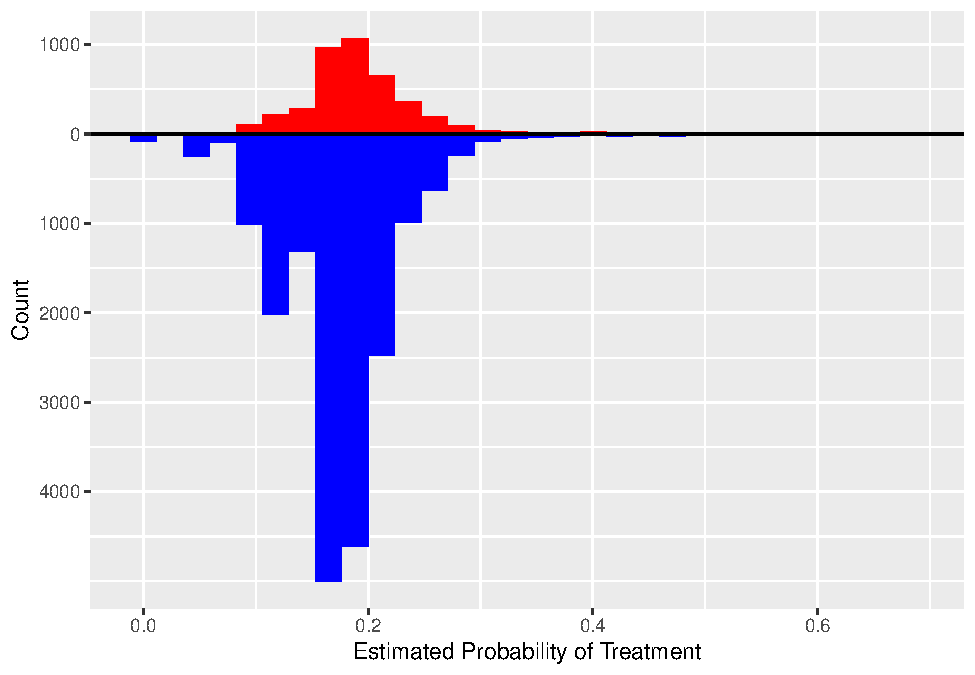
\includegraphics{Paper_files/figure-latex/histpscore-1.pdf}
\caption{\label{fig:histpscore}Distribution of the estimated probability of being sued for the sued (red) and unsued (blue) physicians.}
\end{figure}

\FloatBarrier

\FloatBarrier

\begin{figure}
\centering
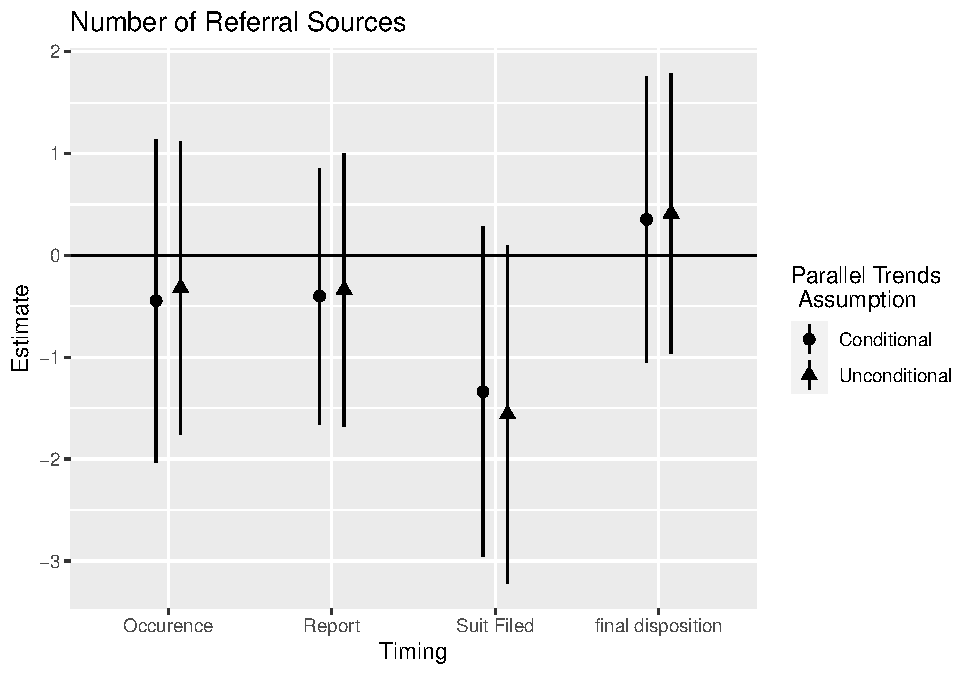
\includegraphics{Paper_files/figure-latex/nsrcatt-1.pdf}
\caption{\label{fig:nsrcatt}Difference-in-differences estimates of the effect of being sued for malpractice on the number of general and primary practice physicians a specialist receives referrals from.}
\end{figure}

\FloatBarrier

\begin{figure}
\centering
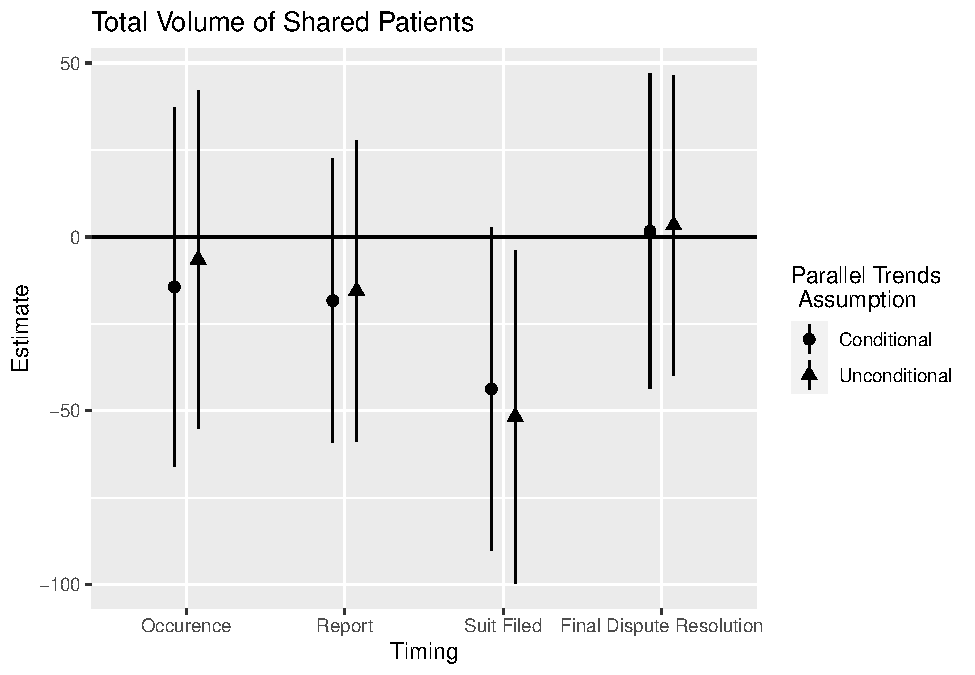
\includegraphics{Paper_files/figure-latex/volatt-1.pdf}
\caption{\label{fig:volatt}Difference-in-differences estimates of the effect of being sued for malpractice on the total volume of patients a specialist shares with general and primary practice physicians.}
\end{figure}

\FloatBarrier

\begin{figure}
\centering
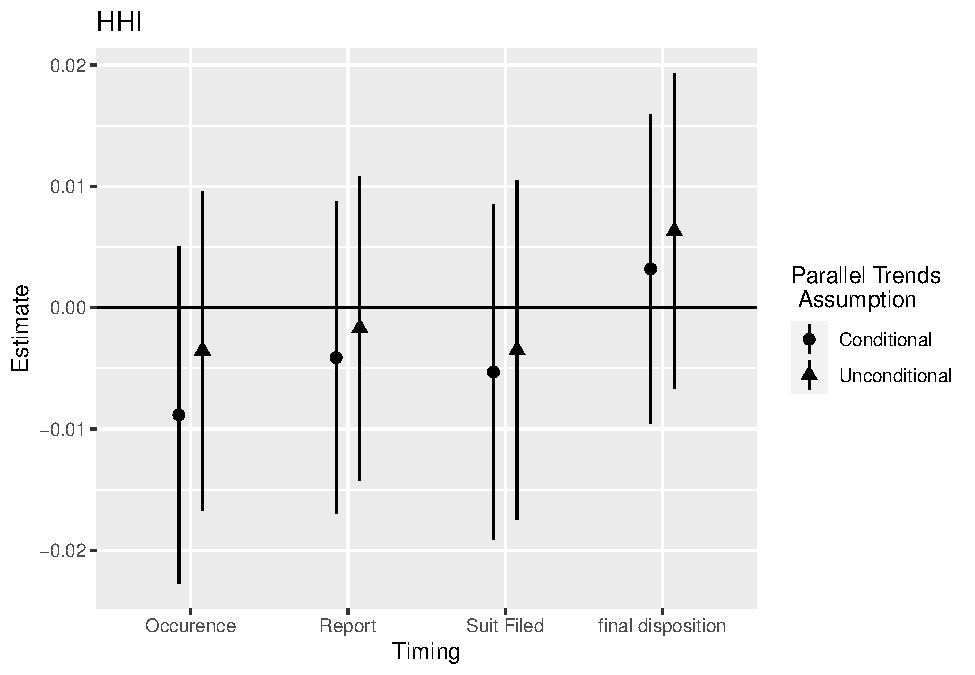
\includegraphics{Paper_files/figure-latex/hhiatt-1.pdf}
\caption{\label{fig:hhiatt}Difference-in-differences estimates of the effect of being sued for malpractice on the concentration of specialists' referrers, as measured by the HHI.}
\end{figure}

\FloatBarrier

\begin{figure}
\centering
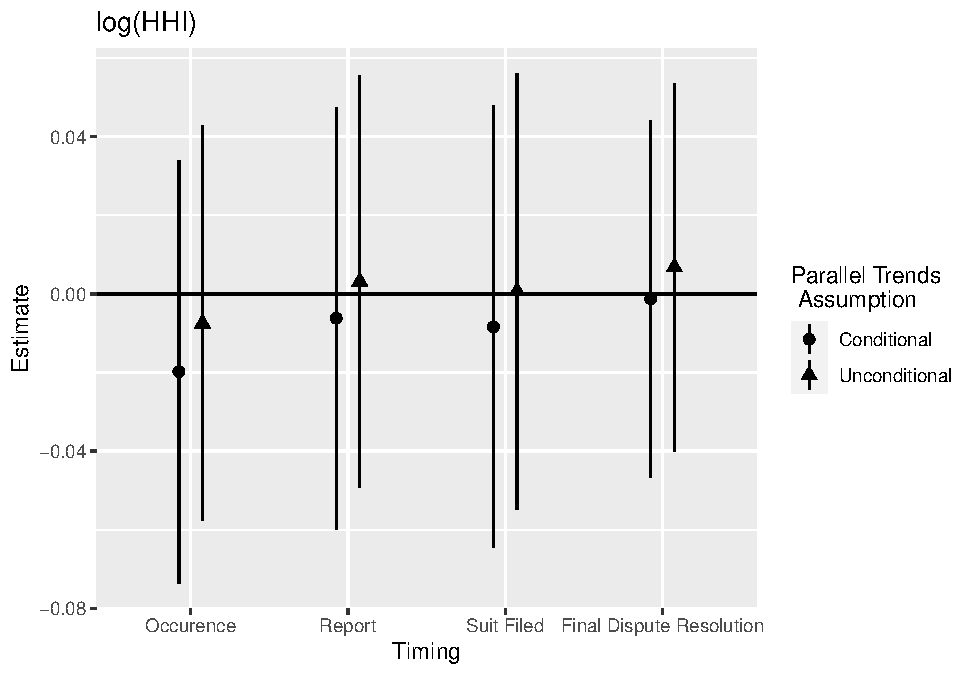
\includegraphics{Paper_files/figure-latex/lhhiatt-1.pdf}
\caption{\label{fig:lhhiatt}Difference-in-differences estimates of the effect of being sued for malpractice on the concentration of specialists' referrers, as measured by log(HHI).}
\end{figure}

\FloatBarrier

\begin{figure}
\centering
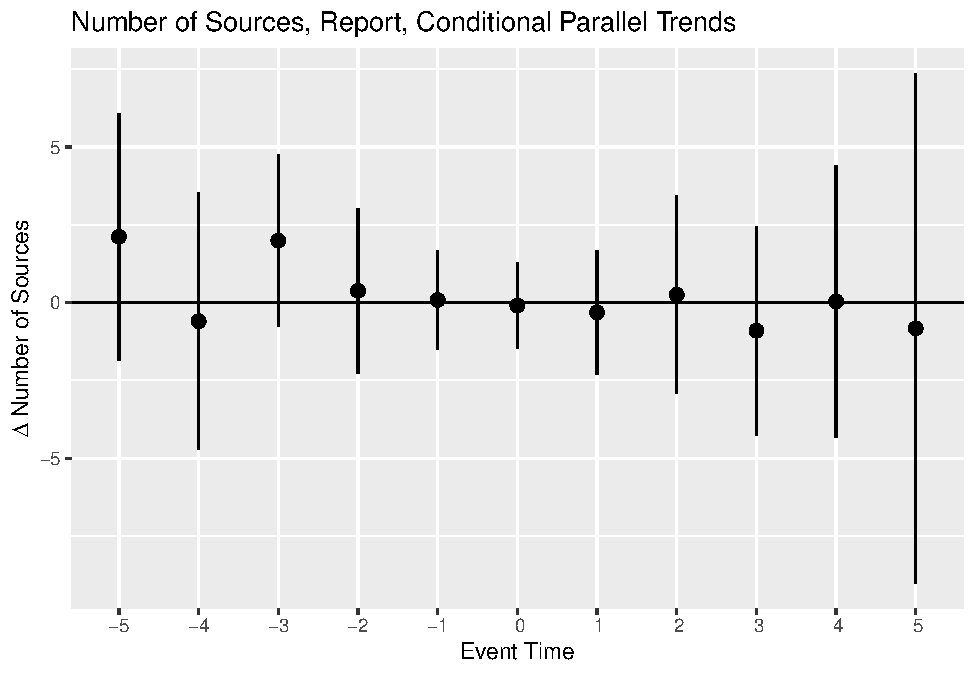
\includegraphics{Paper_files/figure-latex/nsrcrepestud-1.pdf}
\caption{\label{fig:nsrcrepestud}Event study of the effect of being sued on the number of a specialist's referral sources. Here the timing is based on the report date and the parallel trends assumption is conditioned on inpatient volume, PSI rate, and a specialty fixed effect.}
\end{figure}

\FloatBarrier

\begin{figure}
\centering
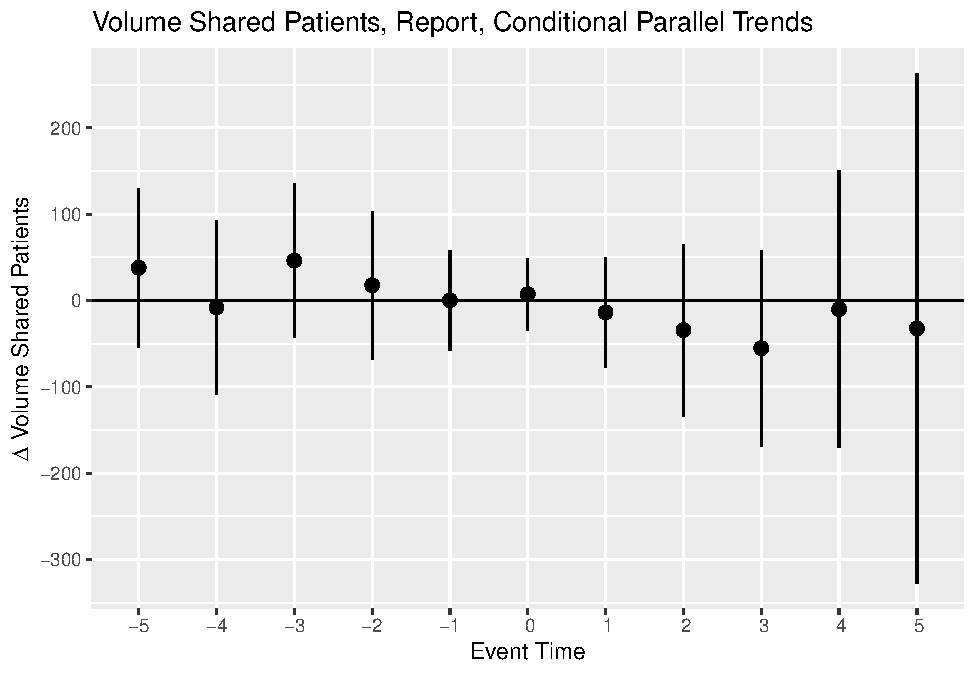
\includegraphics{Paper_files/figure-latex/volrepestud-1.pdf}
\caption{\label{fig:volrepestud}Event study of the effect of being sued on a specialist's volume of shared patients. Here the timing is based on the report date and the parallel trends assumption is conditioned on inpatient volume, PSI rate, and a specialty fixed effect.}
\end{figure}

\FloatBarrier

\begin{figure}
\centering
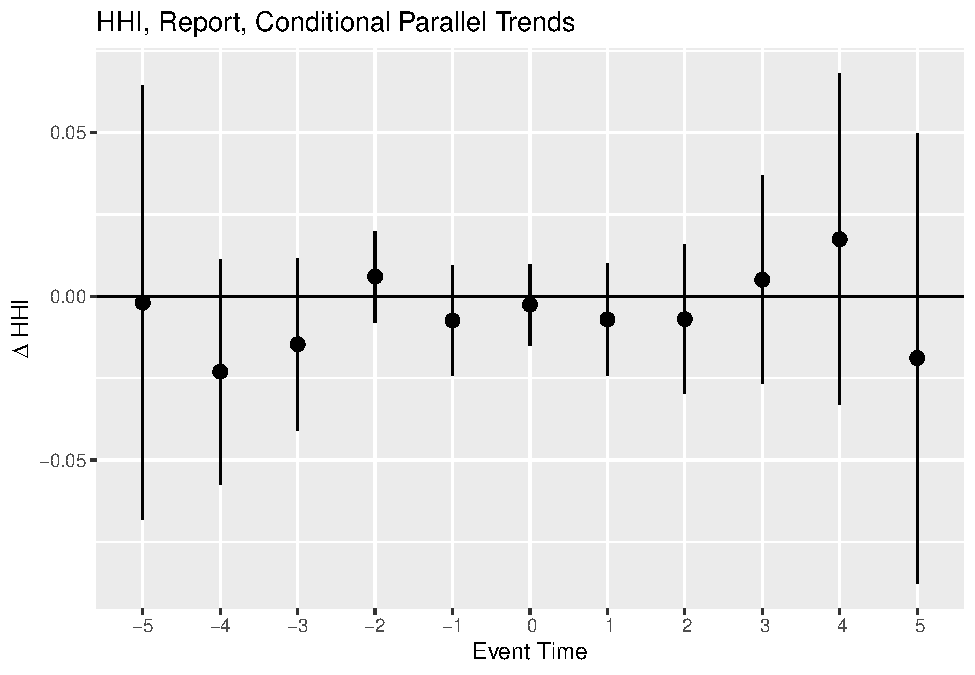
\includegraphics{Paper_files/figure-latex/hhirepestud-1.pdf}
\caption{\label{fig:hhirepestud}Event study of the effect of being sued on the concentration of a specialist's referrals as measured by HHI. Here the timing is based on the report date and the parallel trends assumption is conditioned on inpatient volume, PSI rate, and a specialty fixed effect.}
\end{figure}

\FloatBarrier

\begin{figure}
\centering
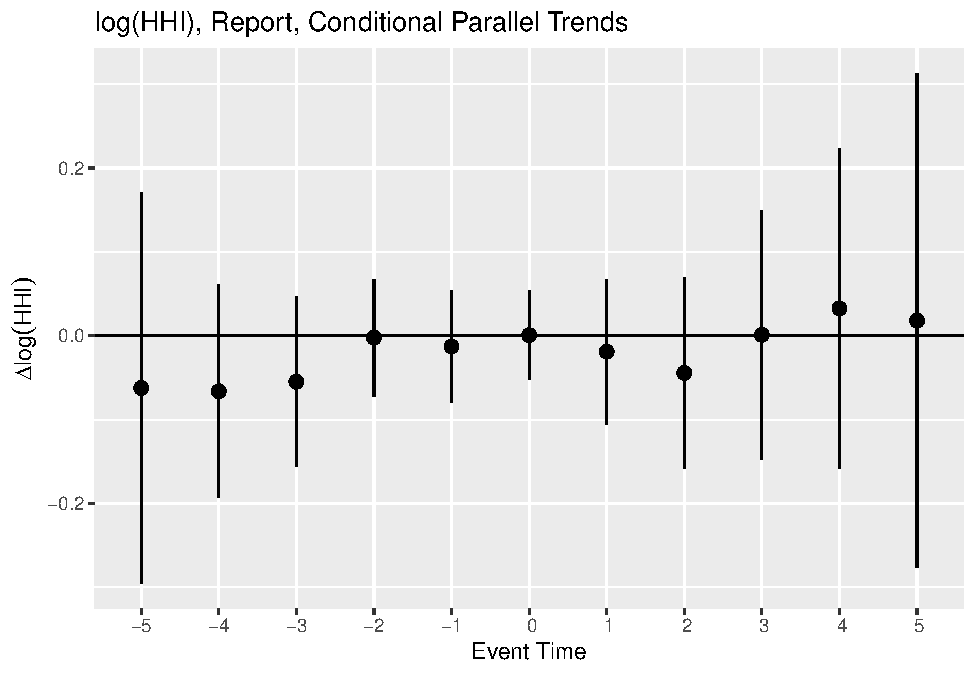
\includegraphics{Paper_files/figure-latex/lhhirepestud-1.pdf}
\caption{\label{fig:lhhirepestud}Event study of the effect of being sued on the concentration of a specialist's referrals as measured by log(HHI). Here the timing is based on the report date and the parallel trends assumption is conditioned on inpatient volume, PSI rate, and a specialty fixed effect.}
\end{figure}

\FloatBarrier

\begin{figure}
\centering
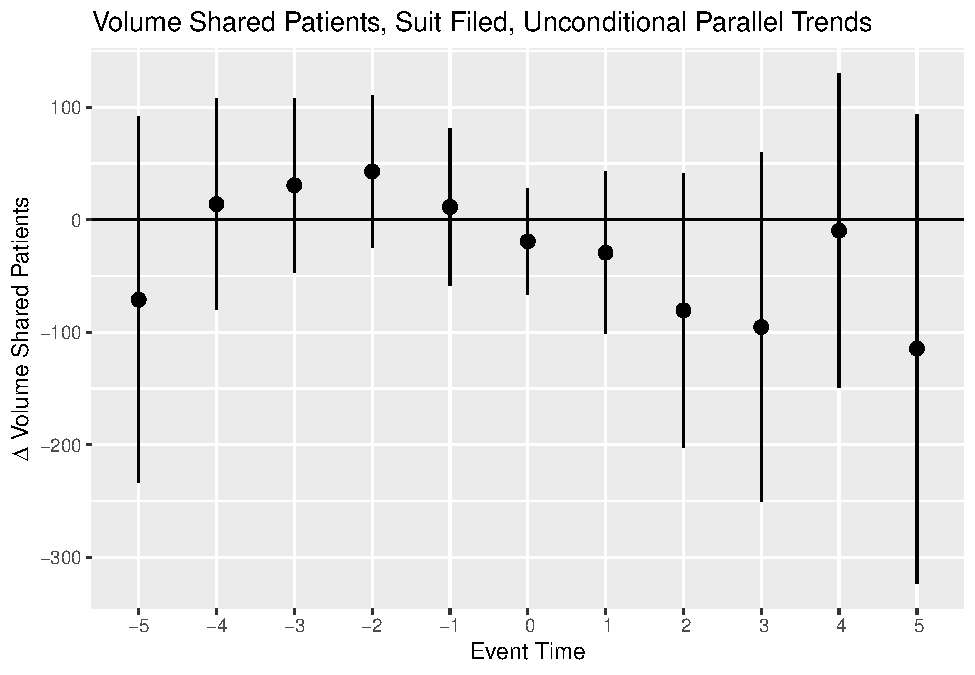
\includegraphics{Paper_files/figure-latex/volsfestud-1.pdf}
\caption{\label{fig:volsfestud}Event study of the effect of being sued on a specialist's volume of shared patients. Here the timing is based on the report date and the parallel trends assumption is not conditioned on any covariates.}
\end{figure}

\end{document}
